\begin{frame}
	\citeA{Heckman.2008a} sets out three tasks for us:
	\begin{itemize}\setlength\itemsep{1em}
		\item Defining the Set of Hypotheticals or Counterfactuals \\\hspace{0.3cm}
		$\Rightarrow$ A Scientific Theory
		\item Identifying Causal Parameters from Hypothetical Population Data \\\hspace{0.3cm}
		$\Rightarrow$ Mathematical Analysis of  Data Point or Set Identification
		\item Identifying Parameters from Real Data\\\hspace{0.3cm}
		$\Rightarrow$ Estimation and Testing Theory
	\end{itemize}
\end{frame}
%-------------------------------------------------------------------------------
%-------------------------------------------------------------------------------
\begin{frame}
\textbf{Parameters of Interest}\\\vspace{0.3cm}
	\begin{itemize}\setlength\itemsep{1em}
		\item conventional average effects
		\item policy-relevant average effects
		\item marginal effects
		\item distributional effects
		\item effects on distributions
	\end{itemize}
\end{frame}
%-------------------------------------------------------------------------------
%-------------------------------------------------------------------------------
\begin{frame}\begin{center}
		\LARGE\textit{Setup}
\end{center}\end{frame}
%-------------------------------------------------------------------------------
%-------------------------------------------------------------------------------
\begin{frame}
	\textbf{The Generalized Roy Model}
	\begin{align*}\begin{array}{l@{\qquad}l}
			\text{Potential Outcomes} &\text{Observed Outcome}\\
			Y_1 = \mu_1(X) + U_1      &  Y = D Y_1 + (1 - D)Y_0 \\
			Y_0 = \mu_0(X) + U_0      &\\
			& \\
			\text{Choice} & \\
			D = \mathrm{I}[\mu_D(X, Z) - V > 0] & \\
		\end{array}
	\end{align*}
\end{frame}
%-------------------------------------------------------------------------------
%-------------------------------------------------------------------------------
\begin{frame}
	\textbf{Useful Notation}
	\begin{align*}
		P(X, Z) & = \Pr(D = 1\mid X, Z) = F_V(\mu_D(X, Z)) \\
		U_D     & = F_V(V)
	\end{align*}
\end{frame}
%-------------------------------------------------------------------------------
%-------------------------------------------------------------------------------
\begin{frame}
	\begin{figure}\caption{First-state unobservable}
		\scalebox{0.35}{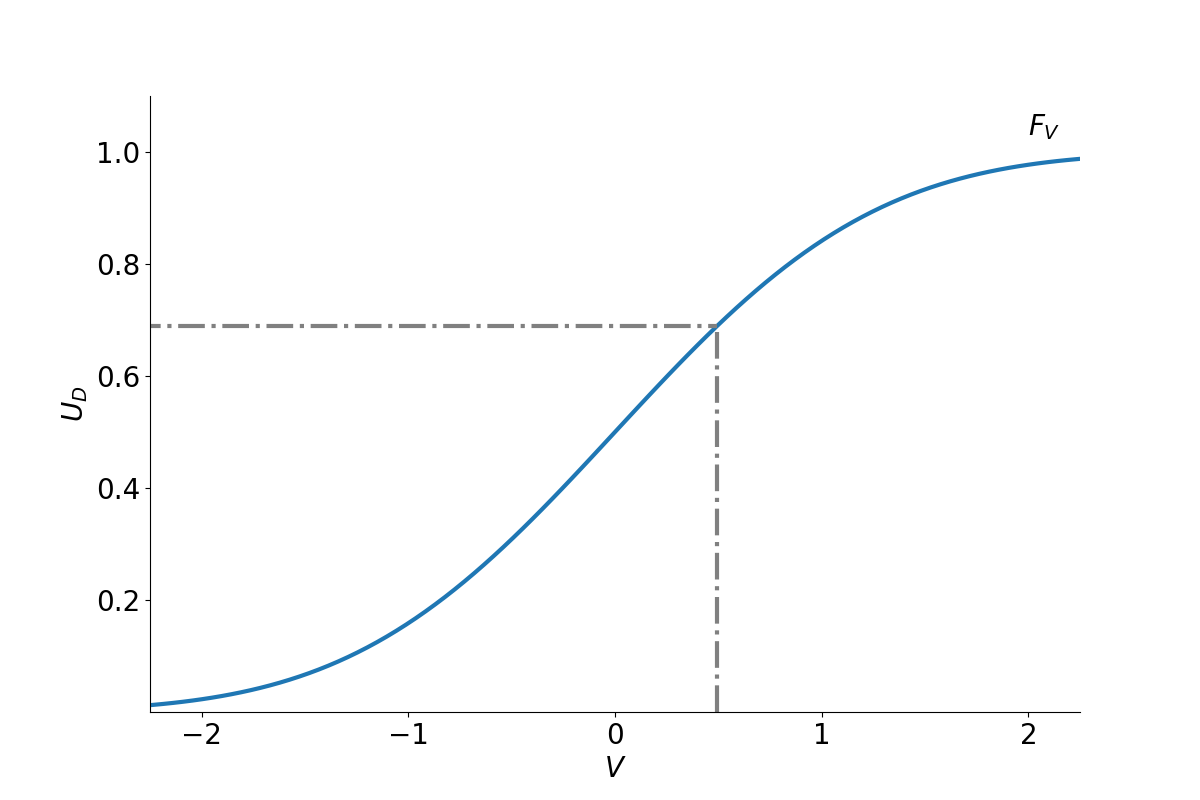
\includegraphics{fig-quantile-function.png}}
	\end{figure}
\end{frame}
